\documentclass[10pt]{article}
\usepackage[T1]{fontenc}
\usepackage{amsmath,amsfonts,times}
\usepackage{graphicx,color,tikz}
\usepackage[paperwidth=17.6cm,paperheight=11.0cm,lmargin=0in,rmargin=0in,tmargin=0.in,bmargin=0.in]{geometry}
\usepackage{bm}
\usetikzlibrary{arrows.meta,shadows,positioning,calc,backgrounds}

\definecolor{cop}{rgb}{0.50,0.20,0.65}
\definecolor{cleaf}{rgb}{0.10,0.35,0.80}
\definecolor{cbad}{rgb}{0.80,0.10,0.10}
\definecolor{cgood}{rgb}{0.05,0.55,0.20}

\tikzset{
  op/.style={draw=black, minimum width=9mm, minimum height=6mm, rectangle, very thick, fill=white, drop shadow, rounded corners=4pt, font=\small, text=cop},
  leaf/.style={draw=black, minimum width=6mm, minimum height=6mm, rectangle, very thick, fill=white, drop shadow, rounded corners=4pt, font=\small, text=cleaf},
  edge/.style={thick, draw=black},
  head/.style={font=\small\bfseries, anchor=west},
  code/.style={font=\scriptsize\ttfamily, anchor=west},
  bar/.style={draw=black, fill=cop!25, thick},
  barleaf/.style={draw=black, fill=cleaf!25, thick},
}

% \stackprofile{heights}{labels}: a bar per clause, the stack depth after it.
\newcommand{\axes}{%
  \draw[-{Stealth[length=2mm]}, thick] (0,0) -- (0,2.35);
  \draw[thick] (0,0) -- (4.55,0);
  \foreach \h in {1,2,3,4} { \draw[black!25] (0,0.5*\h) -- (4.5,0.5*\h); \node[font=\tiny, anchor=east] at (0,0.5*\h) {\h}; }
  \node[font=\scriptsize, rotate=90, anchor=south] at (-0.3,1.1) {values held};
}

\begin{document}
\nopagecolor
\centering
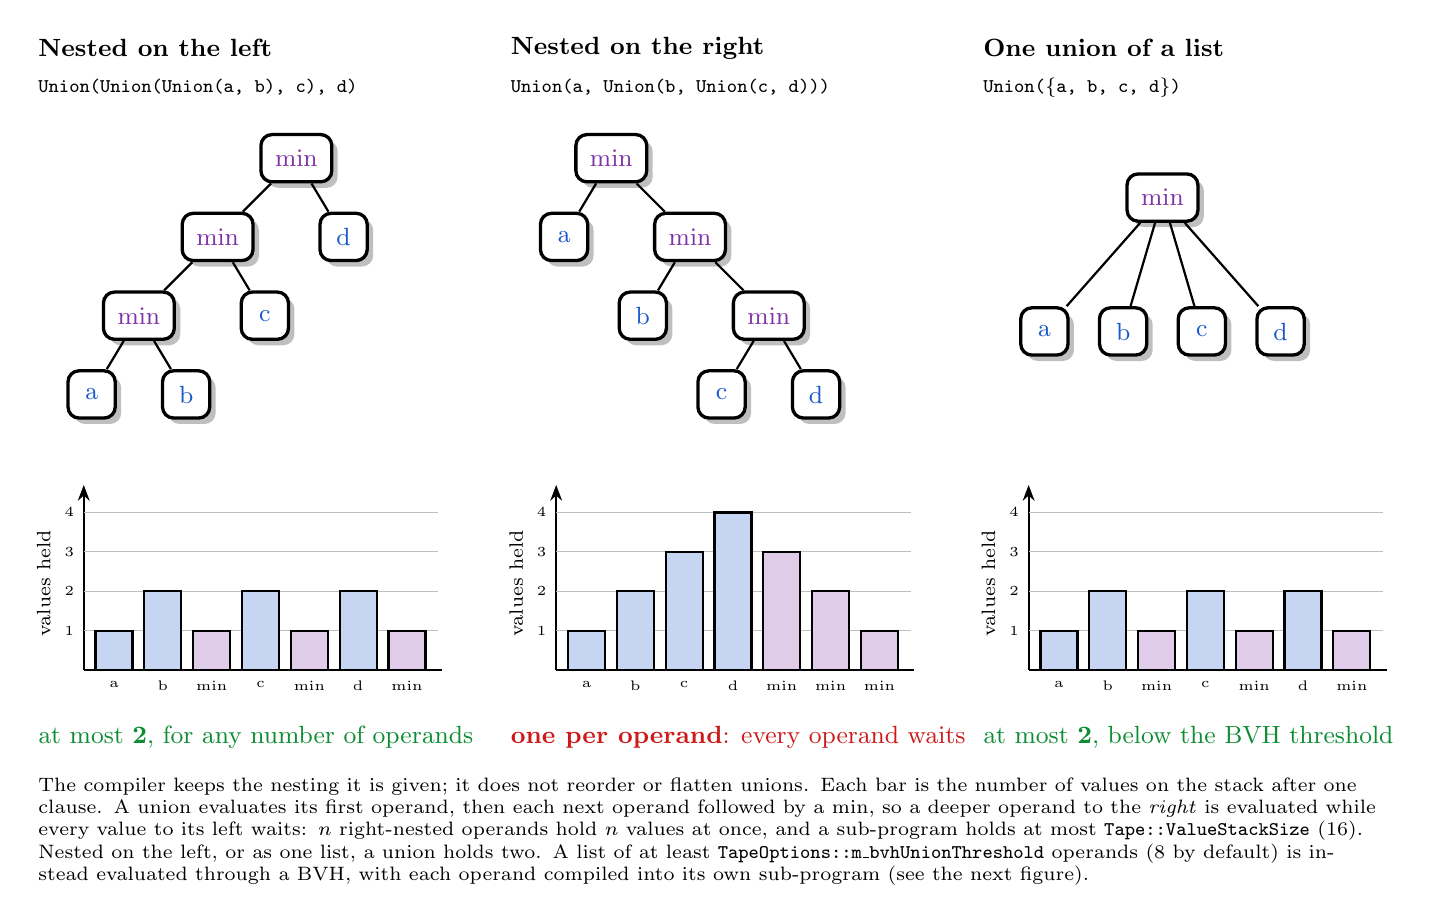
\begin{tikzpicture}[x=1cm, y=1cm]

  % ───────────────────────── Left-nested.
  \begin{scope}[shift={(0.6,0)}]
    \node[head] at (-0.4,10.1) {Nested on the left};
    \node[code] at (-0.4,9.6) {Union(Union(Union(a, b), c), d)};

    \node[op] (u1) at (3.0,8.7) {min};
    \node[op] (u2) at (2.0,7.7) {min};
    \node[op] (u3) at (1.0,6.7) {min};
    \node[leaf] (a) at (0.4,5.7) {a};
    \node[leaf] (b) at (1.6,5.7) {b};
    \node[leaf] (c) at (2.6,6.7) {c};
    \node[leaf] (d) at (3.6,7.7) {d};
    \draw[edge] (u1) -- (u2); \draw[edge] (u1) -- (d);
    \draw[edge] (u2) -- (u3); \draw[edge] (u2) -- (c);
    \draw[edge] (u3) -- (a);  \draw[edge] (u3) -- (b);

    \begin{scope}[shift={(0.3,2.2)}]
      \axes
      \foreach \i/\h/\l/\s in {0/1/a/barleaf, 1/2/b/barleaf, 2/1/min/bar, 3/2/c/barleaf, 4/1/min/bar, 5/2/d/barleaf, 6/1/min/bar} {
        \draw[\s] (0.15+0.62*\i,0) rectangle (0.62+0.62*\i,0.5*\h);
        \node[font=\tiny, anchor=north] at (0.385+0.62*\i,-0.02) {\l};
      }
    \end{scope}
    \node[font=\small, text=cgood, anchor=west] at (-0.4,1.35) {at most \textbf{2}, for any number of operands};
  \end{scope}

  % ───────────────────────── Right-nested.
  \begin{scope}[shift={(6.6,0)}]
    \node[head] at (-0.4,10.1) {Nested on the right};
    \node[code] at (-0.4,9.6) {Union(a, Union(b, Union(c, d)))};

    \node[op] (u1) at (1.0,8.7) {min};
    \node[op] (u2) at (2.0,7.7) {min};
    \node[op] (u3) at (3.0,6.7) {min};
    \node[leaf] (a) at (0.4,7.7) {a};
    \node[leaf] (b) at (1.4,6.7) {b};
    \node[leaf] (c) at (2.4,5.7) {c};
    \node[leaf] (d) at (3.6,5.7) {d};
    \draw[edge] (u1) -- (a); \draw[edge] (u1) -- (u2);
    \draw[edge] (u2) -- (b); \draw[edge] (u2) -- (u3);
    \draw[edge] (u3) -- (c); \draw[edge] (u3) -- (d);

    \begin{scope}[shift={(0.3,2.2)}]
      \axes
      \foreach \i/\h/\l/\s in {0/1/a/barleaf, 1/2/b/barleaf, 2/3/c/barleaf, 3/4/d/barleaf, 4/3/min/bar, 5/2/min/bar, 6/1/min/bar} {
        \draw[\s] (0.15+0.62*\i,0) rectangle (0.62+0.62*\i,0.5*\h);
        \node[font=\tiny, anchor=north] at (0.385+0.62*\i,-0.02) {\l};
      }
    \end{scope}
    \node[font=\small, text=cbad, anchor=west] at (-0.4,1.35) {\textbf{one per operand}: every operand waits};
  \end{scope}

  % ───────────────────────── One n-ary union.
  \begin{scope}[shift={(12.6,0)}]
    \node[head] at (-0.4,10.1) {One union of a list};
    \node[code] at (-0.4,9.6) {Union(\{a, b, c, d\})};

    \node[op] (u) at (2.0,8.2) {min};
    \foreach \n/\x in {a/0.5, b/1.5, c/2.5, d/3.5} {
      \node[leaf] (\n) at (\x,6.5) {\n};
      \draw[edge] (u) -- (\n);
    }

    \begin{scope}[shift={(0.3,2.2)}]
      \axes
      \foreach \i/\h/\l/\s in {0/1/a/barleaf, 1/2/b/barleaf, 2/1/min/bar, 3/2/c/barleaf, 4/1/min/bar, 5/2/d/barleaf, 6/1/min/bar} {
        \draw[\s] (0.15+0.62*\i,0) rectangle (0.62+0.62*\i,0.5*\h);
        \node[font=\tiny, anchor=north] at (0.385+0.62*\i,-0.02) {\l};
      }
    \end{scope}
    \node[font=\small, text=cgood, anchor=west] at (-0.4,1.35) {at most \textbf{2}, below the BVH threshold};
  \end{scope}

  % ───────────────────────── The common footnote.
  \node[anchor=north west, font=\scriptsize, text width=17.0cm, align=left] at (0.2,0.95) {%
    The compiler keeps the nesting it is given; it does not reorder or flatten unions. Each bar is the number of values
    on the stack after one clause. A union evaluates its first operand, then each next operand followed by a $\min$,
    so a deeper operand to the \emph{right} is evaluated while every value to its left waits: $n$ right-nested operands
    hold $n$ values at once, and a sub-program holds at most \texttt{Tape::ValueStackSize} (16). Nested on the left, or
    as one list, a union holds two. A list of at least \texttt{TapeOptions::m\_bvhUnionThreshold} operands (8 by
    default) is instead evaluated through a BVH, with each operand compiled into its own sub-program (see the next figure).%
  };

\end{tikzpicture}

\end{document}
